%%%%%%%%%%%%%%%%%%%%%%%%%%%%%%%%%%%%%%%
% PREMIERE PARTIE
%%%%%%%%%%%%%%%%%%%%%%%%%%%%%%%%%%%%%%%

\section*{Première partie}
\subsection*{Population avant vaccination}
Après avoir lancé la simulation avec une population non vaccinée, nous avons obtenu 
les résultats représentés par les figures \ref{fig:1-1-nb-malades} et \ref{fig:1-1-nb-morts}   

\begin{figure}[htbp] 
%\begin{figure}[h]
  \centering
  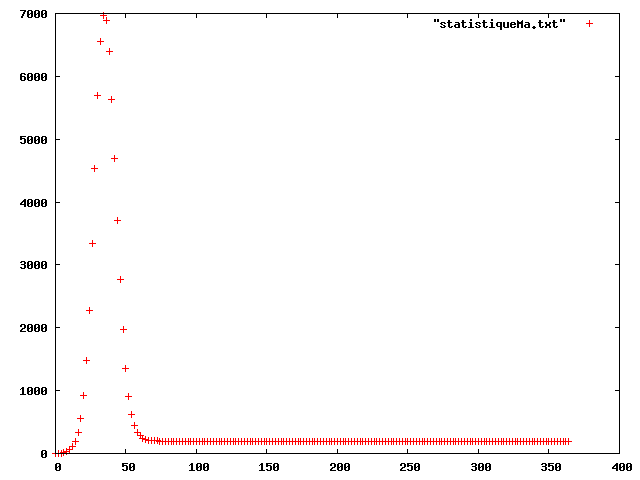
\includegraphics[width=15cm]{1-1-statistiqueMa.png}
  % usecase.png: 985x829 pixel, 72dpi, 34.75x29.25 cm, bb=0 0 985 829
  \caption{Nombre de personnes contaminées par jour}
  \label{fig:1-1-nb-malades}
\end{figure}

\begin{figure}[htbp] 
%\begin{figure}[h]
  \centering
  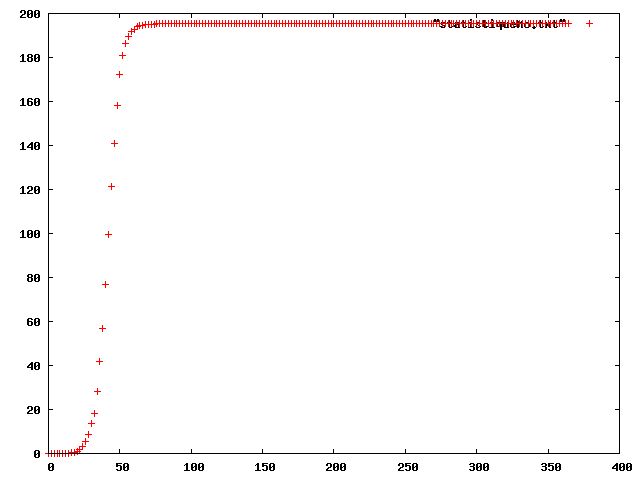
\includegraphics[width=15cm]{1-1-statistiqueMo.png}
  % usecase.png: 985x829 pixel, 72dpi, 34.75x29.25 cm, bb=0 0 985 829
  \caption{Nombre de personnes mortes par jour}
  \label{fig:1-1-nb-morts}
\end{figure}

\subsection*{Population après vaccination}
Dans cette partie, nous avons lancé plusieurs simulations sur des populations dans 
lesquelles  le taux de vaccination valait entre 0\% et 100\%. Les figures  \ref{fig:1-2-nb-malades} 
et \ref{fig:1-2-nb-morts} représentent les résultas obtenus.

\begin{figure}[htbp] 
%\begin{figure}[h]
  \centering
  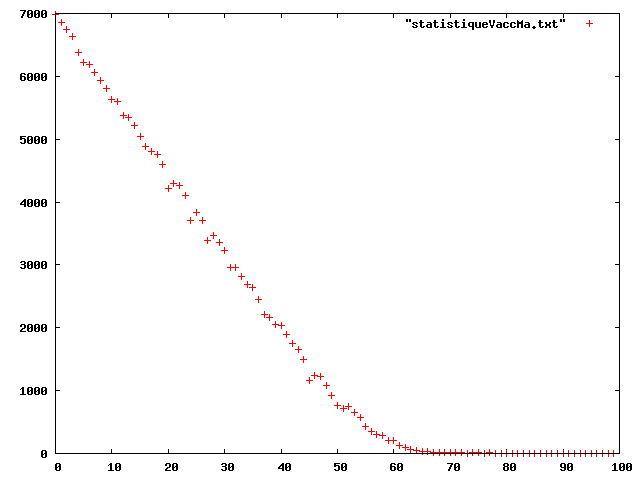
\includegraphics[width=15cm]{1-2-statistiqueMa.png}
  % usecase.png: 985x829 pixel, 72dpi, 34.75x29.25 cm, bb=0 0 985 829
  \caption{Taux de contamination maximal en fonction du pourcentage de population vaccinée}
  \label{fig:1-2-nb-malades}
\end{figure}

 \begin{figure}[h]
  \centering
  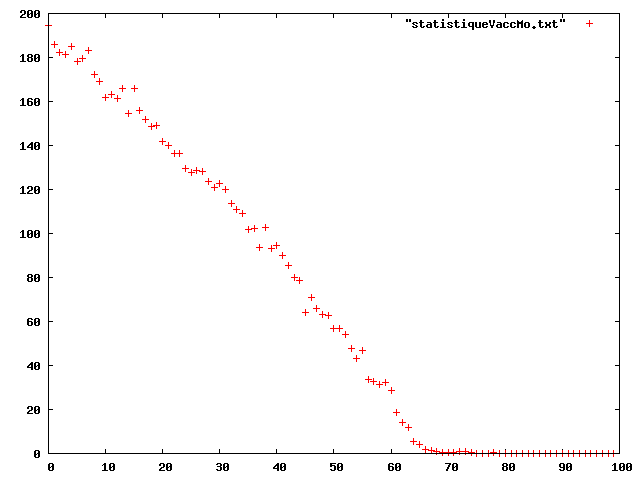
\includegraphics[width=15cm]{1-2-statistiqueMo.png}
  % usecase.png: 985x829 pixel, 72dpi, 34.75x29.25 cm, bb=0 0 985 829
  \caption{Taux de mortalité maximal en fonction du pourcentage de population vaccinée}
  \label{fig:1-2-nb-morts}
\end{figure}
